\documentclass[tikz, border=15pt]{standalone}
\usepackage{amsmath, amssymb, physics}
% Added 'decorations.pathreplacing' to the library list!
\usetikzlibrary{arrows.meta, positioning, shapes.geometric, calc, fit, backgrounds, decorations.pathreplacing}

\begin{document}

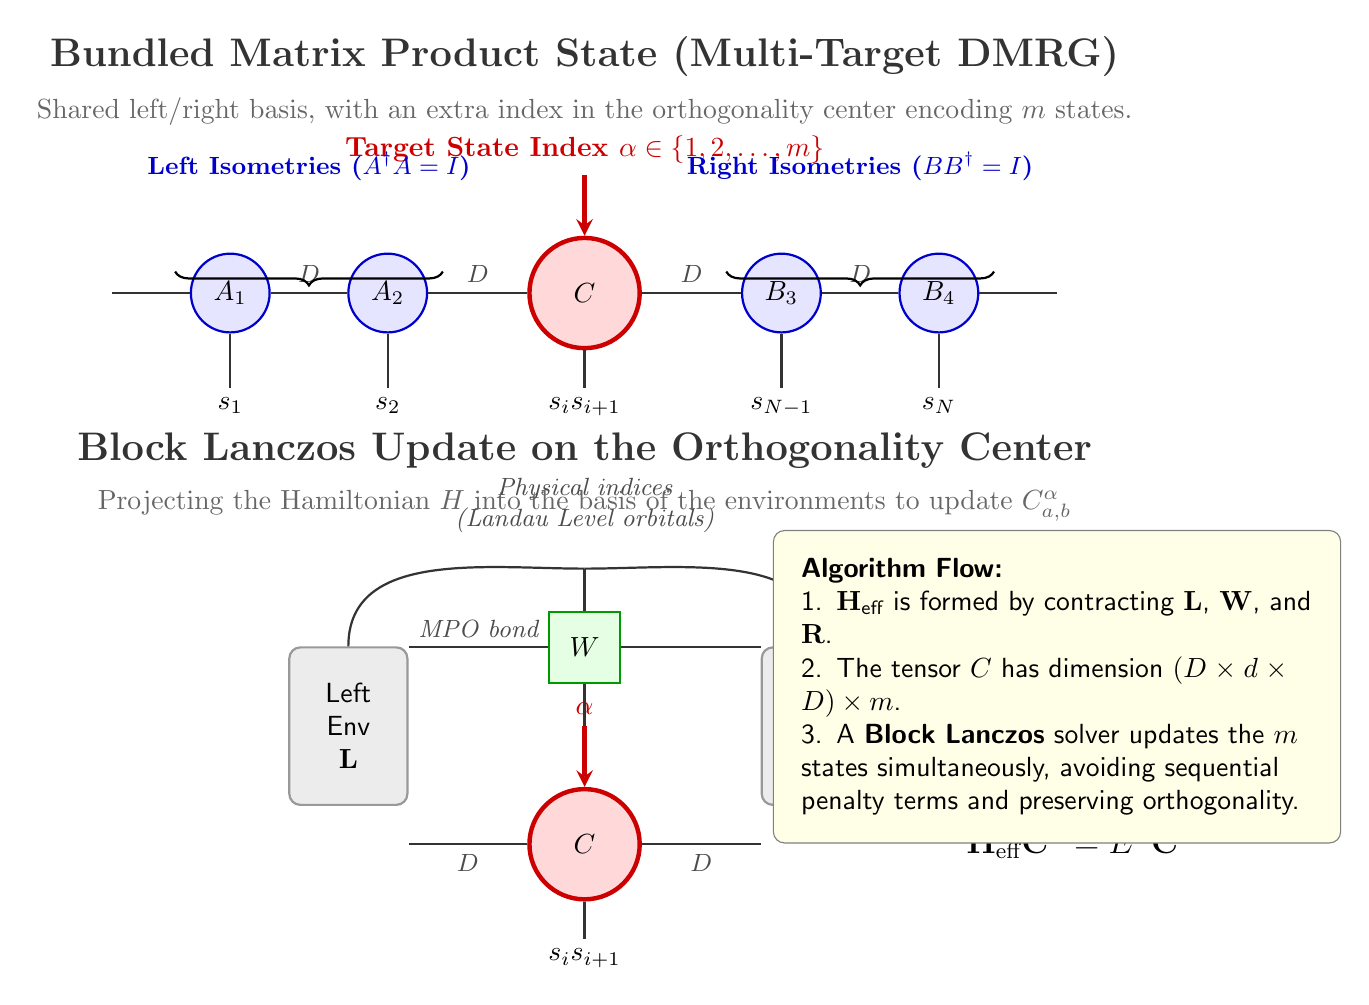
\begin{tikzpicture}[
    >=stealth, font=\sffamily,
    mps/.style={circle, draw=blue!80!black, fill=blue!10, thick, minimum size=1cm, inner sep=0},
    center/.style={circle, draw=red!80!black, fill=red!15, ultra thick, minimum size=1.4cm, inner sep=0},
    mpo/.style={rectangle, draw=green!60!black, fill=green!10, thick, minimum size=0.9cm, inner sep=0},
    env/.style={rectangle, rounded corners, draw=gray!80, fill=gray!15, thick, minimum width=1.5cm, minimum height=2cm, align=center},
    leg/.style={thick, draw=black!80},
    targetleg/.style={ultra thick, draw=red!80!black, <-},
    label text/.style={font=\small\itshape, text=black!70}
]

    % =========================================================
    % PART 1: THE BUNDLED MPS REPRESENTATION
    % =========================================================
    \node[font=\Large\bfseries, text=black!80] at (0, 3) {Bundled Matrix Product State (Multi-Target DMRG)};
    \node[font=\normalsize, text=gray!80!black] at (0, 2.3) {Shared left/right basis, with an extra index in the orthogonality center encoding $m$ states.};

    % Tensors
    \node[mps] (A1) at (-4.5, 0) {$A_1$};
    \node[mps] (A2) at (-2.5, 0) {$A_2$};
    \node[center] (C) at (0, 0) {$C$};
    \node[mps] (B1) at (2.5, 0) {$B_3$};
    \node[mps] (B2) at (4.5, 0) {$B_4$};

    % Virtual Bonds (Horizontal)
    \draw[leg] (-6, 0) -- (A1) node[midway, above, label text] {};
    \draw[leg] (A1) -- (A2) node[midway, above, label text] {$D$};
    \draw[leg] (A2) -- (C) node[midway, above, label text] {$D$};
    \draw[leg] (C) -- (B1) node[midway, above, label text] {$D$};
    \draw[leg] (B1) -- (B2) node[midway, above, label text] {$D$};
    \draw[leg] (B2) -- (6, 0) node[midway, above, label text] {};

    % Physical Bonds (Vertical Down)
    \foreach \name/\pos/\index in {A1/-4.5/s_1, A2/-2.5/s_2, C/0/s_i s_{i+1}, B1/2.5/s_{N-1}, B2/4.5/s_N} {
        \draw[leg] (\name) -- (\pos, -1.2) node[below] {$\index$};
    }
    \node[below=1.5cm of C, label text, text width=4cm, align=center] {Physical indices \\ (Landau Level orbitals)};

    % Target State Bond (Vertical Up - Key Innovation)
    \draw[targetleg] (C) -- (0, 1.5) node[above, text=red!80!black, font=\bfseries] {Target State Index $\alpha \in \{1, 2, \dots, m\}$};

    % Left and Right Orthogonal Isometries labels (This is where the decoration error occurred)
    \draw[decorate, decoration={brace, amplitude=5pt, raise=1.5ex}, thick] (-1.8, 0.5) -- (-5.2, 0.5) node[midway, above=0.8cm, font=\small\bfseries, text=blue!80!black] {Left Isometries ($A^\dagger A = I$)};
    \draw[decorate, decoration={brace, amplitude=5pt, raise=1.5ex}, thick] (5.2, 0.5) -- (1.8, 0.5) node[midway, above=0.8cm, font=\small\bfseries, text=blue!80!black] {Right Isometries ($B B^\dagger = I$)};

    % =========================================================
    % PART 2: BLOCK LANCZOS UPDATE (EFFECTIVE HAMILTONIAN)
    % =========================================================
    
    \begin{scope}[yshift=-6cm]
        \node[font=\Large\bfseries, text=black!80] at (0, 4) {Block Lanczos Update on the Orthogonality Center};
        \node[font=\normalsize, text=gray!80!black] at (0, 3.3) {Projecting the Hamiltonian $H$ into the basis of the environments to update $C^\alpha_{a,b}$};

        % Center Tensor C
        \node[center] (C_eff) at (0, -1) {$C$};
        \draw[targetleg] (C_eff) -- (0, 0.5) node[above, text=red!80!black, font=\bfseries] {$\alpha$};
        \draw[leg] (C_eff) -- (0, -2.2) node[below] {$s_i s_{i+1}$};

        % MPO (Hamiltonian)
        \node[mpo] (W) at (0, 1.5) {$W$};
        \draw[leg] (W) -- (0, 2.5); % Top physical 
        \draw[leg] (W) -- (0, 0.5); % Connects down to C

        % Left Environment
        \node[env] (L) at (-3, 0.5) {Left \\ Env \\ $\mathbf{L}$};
        % Right Environment
        \node[env] (R) at (3, 0.5) {Right \\ Env \\ $\mathbf{R}$};

        % Connect environments to MPO and C
        % Top virtual bonds (MPO level)
        \draw[leg] (L.east |- W) -- (W) node[midway, above, label text] {MPO bond};
        \draw[leg] (W) -- (R.west |- W);
        
        % Bottom virtual bonds (MPS level)
        \draw[leg] (L.east |- C_eff) -- (C_eff) node[midway, below, label text] {$D$};
        \draw[leg] (C_eff) -- (R.west |- C_eff) node[midway, below, label text] {$D$};

        % Connecting lines bending from environments to top open physical legs 
        \draw[leg] (L.north) to[out=90, in=180] (0, 2.5);
        \draw[leg] (R.north) to[out=90, in=0] (0, 2.5);

        % Equation Text
        \node[right=4cm of C_eff, font=\large] {$\displaystyle \mathbf{H}_{\text{eff}} \mathbf{C}^\alpha = E^\alpha \mathbf{C}^\alpha$};
        
        % Annotation Box
        \node[draw=black!50, fill=yellow!10, rounded corners, inner sep=10pt, text width=6.5cm, align=left] at (6, 1) {
            \textbf{Algorithm Flow:}\\
            1. $\mathbf{H}_{\text{eff}}$ is formed by contracting $\mathbf{L}$, $\mathbf{W}$, and $\mathbf{R}$.\\
            2. The tensor $C$ has dimension $(D \times d \times D) \times m$.\\
            3. A \textbf{Block Lanczos} solver updates the $m$ states simultaneously, avoiding sequential penalty terms and preserving orthogonality.
        };

    \end{scope}

\end{tikzpicture}

\end{document}
